


\section{Zielsetzung}
Ziel des Versuchs ist die Bestimmung des Wirkungsquerschnittes $\sigma$,
bzw des Absorptionskoeffizienten $\mu = n\sigma$, wobei n die Zahl der Materieteilchen ist.
\section{Theorie}
Für diesen Versuch wird die Wechelwirkungen ernergiereicher Strahlung mt Materie betrachtet.
Dafür wird zum einen $\gamma$-Strahlung als Photonen-Strahlung,
zum anderen $\beta^-$-Strahlung als Teilchen-Strahlung von instabielen Kernen betrachtet.
Beim Durchgang durch Materie tritt bei einem $\gamma$-Quant nur eine Wechelwirkung auf,
wogegen bei den $\beta$-Teilchen viele Prozesse nacheinander auftreten bis die kinetische Energie verbraucht ist.\\
Trifft ein Teilchenstrahl auf eine Materieschicht nimmt durch die Wechselwirkungen die Intensität ab.
Der Wirkungsquerschnitt $\sigma$ ist ein Maß für die Häufigkeit der Wechselwirkungen.
Die Wahrscheinlichkeit, dass durch ein Teilchen Wechelwirkungen stattfinden, wird beschrieben durch

\begin{equation}
  W = nD\sigma
\end{equation}
Dabei ist D die Dicke.\\
Das Absorptionsgesetz
\begin{equation}
  N(D)= N_0 e^{-n\sigma D}
\end{equation}
gilt, wenn jedes Teilchen durch eine Wechselwirkung vernichtet wird oder
die mittlere Abstand zwischen zwei Reaktionen sehr groß ist.
Der Absorptionskoeffizient $\mu = \sigma n$ kann durch die Absorptionsmessung bestimmt werden.\\
Die Anzahl der Teilchen im Absorber wird mit
\begin{equation}
  n = \frac{zN_L}{V_mol} = \frac{zN_L\rho}{M}
\end{equation}
berechnet.
Dabei ist $N_L$ die Loschmidtsche Zahl, $V_mol$ das Molvolumen und M das Molekulargewicht.

\section{Gamma-Strahlung}
Die Elektronenhülle und die Atomkerne besitzen diskrete Energieniveaus.
Wird eine große Zahl von Quanten über die Zeit und den Raum gemiitelt, ergeben sich Eigenschaften,
die einer Elektromagnetischen Welle ähneln.
Somit ergibt sich für die Energie :
\begin{equation}
  E = h\frac{c}{\lambda}
\end{equation}
Dabei ist h das Plancksche Wirkungsquantum, c die Lichtgeschwindigkeit und $\lambda$ die Wellenlänge.\\
Tritt ein $\gamma$-Quant in eine Materieschicht ein, kommt es zu Wechselwirkungen.
Am Häufigsten treten diese bei Energien zwischen 10\,keV und 10\,MeV.
Es wird zwischen Annihilationsprozessen, inelastischer Streuung und elastischer Streuung unterschieden.
Bei Annihilation verschwindet der $\gamma$-Quant.
Prozesse, in denen dieses auftritt sind zum einen der Photoeffekt,
 bei dem das $\gamma$-Quant bei Wechselwirkungen mit einem Hüllenelektron vernichtet und das Elektron aus seiner Bindung entfernt wird,
  und zum anderen die Paarbildung,
 dass die Umwandlung eines Photons in ein Elektron-Positron-Paar beschreibt.
 Bei elastischer Streuung tritt eine Richtungsänderung der qunten auf.
Bei inelastischer Streuung tritt eine Änderung der Richtung auf
und der $\gamma$-Quant gibt einen Teil seiner Energie an seinen stoßpartner ab.
Dieses wird beim Comptoneffekt beobachtet.
Der Effekt führt zu einer Intesitätsabnahme eines $\gamma$-Strahls, da die Quanten in unterschiedliche Richtungen abgelengt werden.
Somit nimmt auch die zahl der Quanten pro Fläche und Zeit ab.
Der wirkungsquerschnitt $\sigma_{com}$ ergibt sich zu
\begin{equation}
  \sigma_{com} = 2\pi r_e^2\left(\frac{1 + \varepsilon}{\varepsilon^2}\left(\frac{2(1+\varepsilon)}{1+2\varepsilon}-\frac{1}{\varepsilon}
  ln(1+2\varepsilon)\right)+\frac{1}{2\varepsilon}ln(1+2\varepsilon)-\frac{1+3\varepsilon}{(1+2\varepsilon)^2}\right).
  \label{eqn:sigma}
\end{equation}
Dabei ist $r_e$ der klassische Elektronenradius und $\varepsilon$ das Verhältnis der Quantenenergie $E_{\gamma}$ zur Ruheenergie des Elektrons.\\
für kleine Enrgien $E_{\gamma}$ wird $\sigma_{com}$ enrgieunabhängig.
Durch den Comptoneffekt ist ein Absorptionskoeffizient $\mu_{com}$ bedingt.
Dieser ergibt sich zu
\begin{equation}
  \mu_{com} = n \sigma_{com}(\varepsilon) .
  \label{eqn:absorption}
\end{equation}

\section{Beta-Strahlung}

Die $\beta$-Strahlung besteht aus negativen oder Positiven Elektronen.
Die $\beta$-Teilchen entstehen durch Umwandlung eines Nukleons.
Dies kann auf zwei Unterschiedliche Wege erfolgen:
\begin{align*}
  n &\rightarrow p +\beta^- +\bar{\nu}_e \\
  p &\rightarrow n +\beta^- +\nu_e
\end{align*}.
Neben dem Elektron wird ein Neutrino $\nu_e$ bzw ein Antineutrino $\bar{\nu}_e$ emittiert.
Das Neutrino hat einen Spin von \sfrac{1}{2}, eine Ladung von Null und eine Ruhemasse, die kleiner als 1\,eV ist.
Das $\beta$-Teilchen tritt durch seine Ladung und geringe Masse in Wechslwirkung mit Materie,
wenn es in eine Materieschicht eindringt.
Dieser Wechselwirkungsmechanismus wird auch Rutherford-Streuung genannt.
Durch das Coulomb-Feld der Kerne werden die $\beta$-Teilchen aus ihrer Bahnrichtung abgelengt.
dadurch werden die parallelen Strahlenbündel aufgefächert und es kommt zu einer Intesnitätsabnahme.\\
Durch inelastische Streuung im Coulomb-Feld werden die $\beta$-Teilchen beschleunigt.
Die Emission von Photonen führt zu einer Abbremsung der $\beta$-Teilchen.
Diese so entstehende Strahlung wird als Bremsstrahlung bezeichnet.
Die Warscheinlichkeit, dass dieser Prozess eintritt wird mit durch den Wirkungsquerschnitt $\sigma_{Br}$  beschrieben.
\begin{equation}
  \sigma_{Br} = \alpha r_e^2 z^2
\end{equation}
Dabei ist $\alpha$ die Sommerfeldsche Feinstrukturkonstante und $r_e$ der klassische Elektronenradius.
Wenn die Strahlung inelastisch am Elektron gestreut wird, werden die Absorberatome ionisiert und angeregt.\\

Die Absorptionskurve eines natürlichen $\beta$-Strahlers ist in Abbildung \ref{fig:absorb} zu sehen.
\begin{figure}
  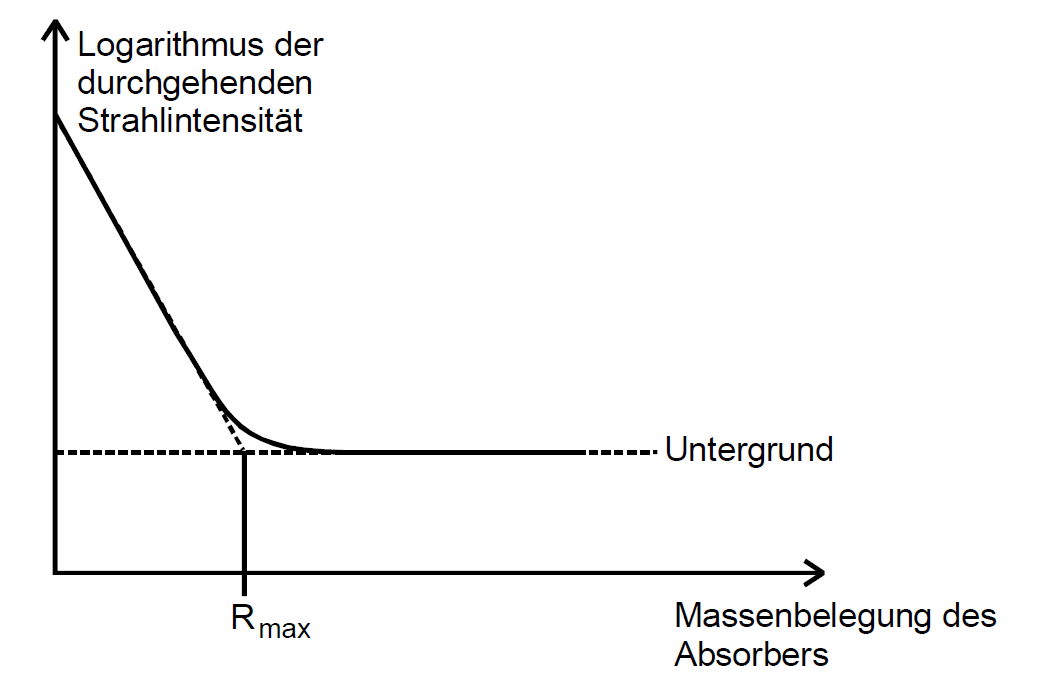
\includegraphics[width=\textwidth]{3.png}
  \caption{Absorptionskurve für einen natürlichen $\beta$-Strahler}\cite{anleitung}
  \label{fig:absorb}
\end{figure}
Oberhalb $R_{max}$ ist die Intensität unabhängig von der Schichtdicke.
Das iegt an der Bremsstrahlung, die durchdringender ist als die $\beta$-Strahlung.
Mit der Absortionskurve, kann $R_{max}$ bestimmt werden.
Dann ergibt sich die beim $\beta$-Zerfall gesamte frei werdende Energie zu
\begin{equation}
  E_{max}=1,92\sqrt{R_{max}^2+0,22R_{max}}
  \label{eqn:E}
\end{equation}

\section{Durchführung}

Zunächst werden die zu verwendenden Materialien ausgemessen.
Die Messung wird zum einen mit dem Beta-Strahler durchgeführt.
Dafür wird der Beta-Strahler in den Versuchsaufbau eingebaut.
Es werden für unterschiedlich dicke Aluminiumplatten,
die ebenfalls in den Versuchsaufbau gesteckt werden, die Zählraten aufgenommen.

Weiter wird der Versuch mit einem Gamma-Strahler durchgeführt.
Hier werden zum einen Zink-Platten und zum anderen Blei-Platten eingebaut.\\
Der Versuchsaufbau ist in Abbildung 8 zu sehen.

\begin{figure}
  \centering
  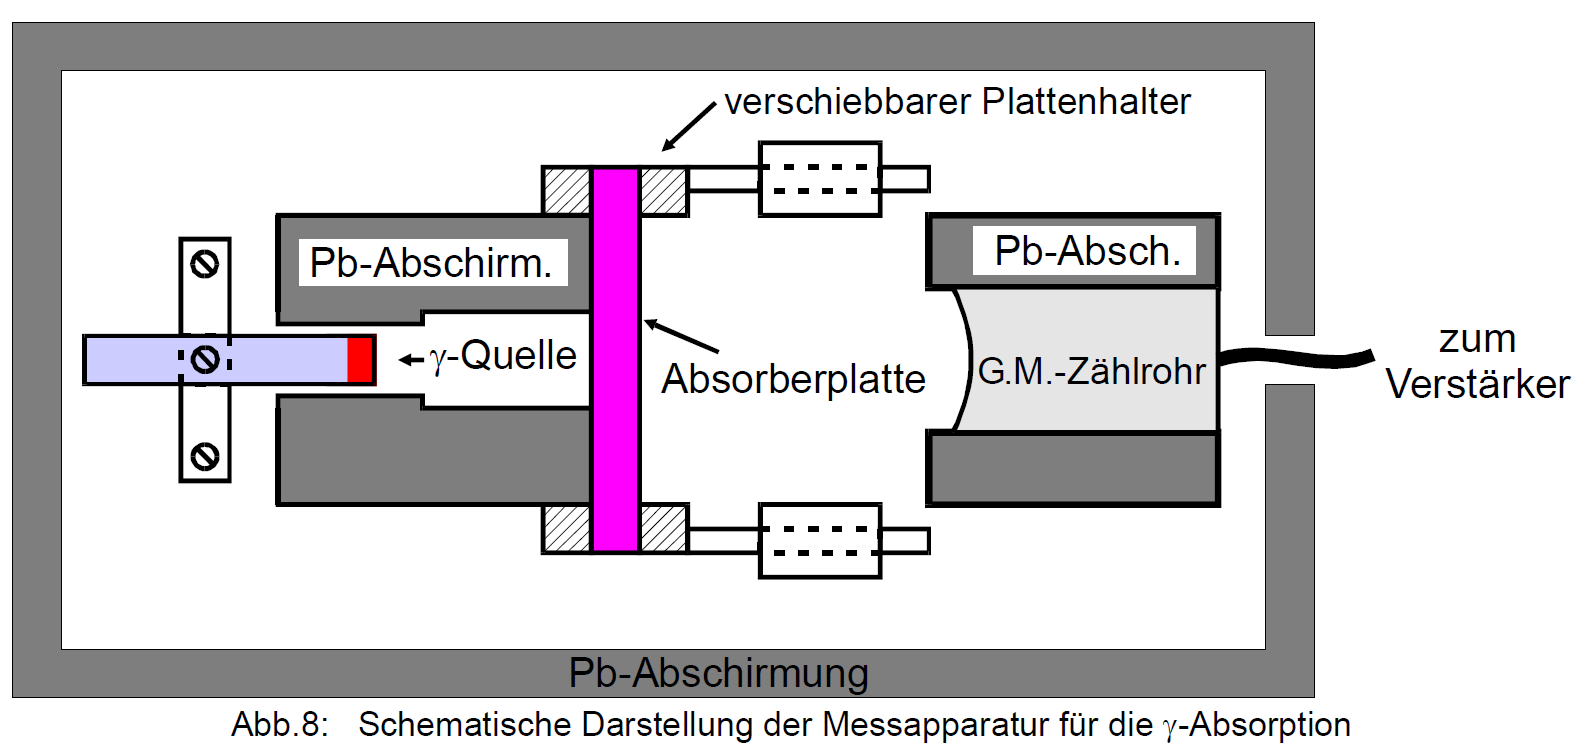
\includegraphics[width=\textwidth]{4.png}
  \cite{anleitung}%\caption{Versuchsaufbau}
  \label{fig:aufbau}
\end{figure}
